\textit{Incoming commands} are commands in a provider application (namely in an application which receives commands from a service user) and \textit{incoming reports} are reports in a user application (namely in an application which receives reports from a service provider).

Incoming commands and incoming reports are treated together because their management is performed in a similar way. 

The management model specified by the framework for incoming commands and reports is based on the definition of the following components:
\begin{itemize}
\item \textbf{InCommand} 
This component models the generic behaviour of a command on a provider application (namely of an incoming command). Concrete incoming commands are defined as extensions of the base InCommand component.
\item \textbf{InReport}
This component models the generic behaviour of a report on a user application (namely of an incoming report). Concrete incoming reports are defined as extensions of the base InReport component.
\item \textbf{InStream}
This component models the interface through which incoming commands and reports are received by an application. 
\item \textbf{InFactory}
The InStream delivers an incoming command or incoming report as a packet consisting of a stream of bytes which must be deserialized to create an InCommand or InReport instance to represent it. The InFactory component encapsulates the component instance creation process.
\item \textbf{InLoader}
This component is responsible for retrieving packets which become available at the InStreams. The InLoader may either forward an incoming packet (if its destination is not the host application), or it may process it as an incoming report (if the packet holds a report), or it may process it as an incoming command (if the packet holds a command). The processing of incoming commands or reports is as follows. The InLoader deserializes the packet and creates an InCommand or InReport instance to represent it and then loads it into an InManager. The InManager will be responsible for executing the InCommand or InReport.
\item \textbf{InManager}
This component controls the execution of an incoming command or incoming report until all its actions have been completed.
\item \textbf{InRegistry}
This component acts as a registry for pending InCommand and InReport. It can provide information about their state to other parts of the applications.  
\end{itemize}

Note that InFactory, InLoader, InRegistry and InStream are singletons and it is
therefore assumed that only one instance of each exists in an application. 

\begin{figure}[h]
 \centering
 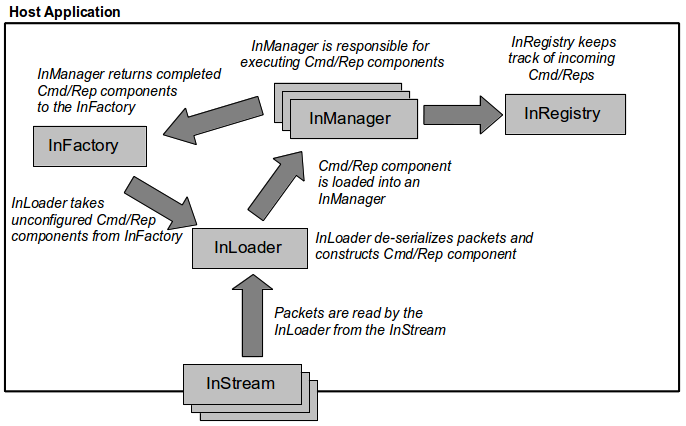
\includegraphics[scale=0.45,keepaspectratio=true]{IncomingCmdAndRep.png}
 \caption{The Management of Incoming Commands and Reports}
 \label{fig:IncomingCmdAndRep}
\end{figure}

The process through which an application processes an incoming command or incoming report is shown using an information notation in figure \ref{fig:IncomingCmdAndRep} and can be summarized as follows:
\begin{enumerate}
\item The InStreams receive packets from other applications. The packets are collected from the InStreams by the InLoader.
\item The InLoader checks the destination of the packet. If it is the host application itself (namely the application within which the InLoader is running), it processes the packet as described below. If it is another application, the InLoader forwards the packet to another application (either its eventual destination or a routing application on the way to its eventual application).
\item An incoming packet may represent either a command or a report. The InLoader identifies the type of the command or report and asks the InFactory to provide an instance of an InCommand (if the packet represents a command) or of an InReport (if the packet represents a report) of that type. 
\item The InCommand or InReport are initially unconfigured. They are configured by deserializing the packet representing the incoming command or incoming report. Henceforth the incoming command or report is represented by the configured InCommand or InReport instance. 
\item The InLoader loads the command or report into an InManager. The InManager is responsible for executing the command or report. In the case of incoming commands, this may require several execution cycles. In the case of incoming reports, at most one execution cycle is sufficient. Depending on the outcome of the conditional checks associated to the incoming command or report, execution may result either in a normal termination or in the command or report being aborted.
\item When the command or report has terminated execution or has been aborted, the InManager returns the InCommand or InReport component instance that held it to the InFactory.
\item The InRegistry is notified of the arrival of incoming commands and reports and of changes of their state. The Inregistry makes this information available to other parts of the host application.
\end{enumerate}

